\documentclass[conference]{IEEEtran}
\usepackage[T1]{fontenc}
\usepackage{graphicx}
\usepackage{booktabs}
\usepackage{amsmath}
\usepackage[hidelinks]{hyperref}
\usepackage{xcolor}
\newcommand{\pending}[1]{\textcolor{red}{#1}}

\begin{document}

\title{Detecting Breast Cancer Lymph Node Metastases in Histopathology Patches: Dataset and Baseline Results}

\author{\IEEEauthorblockN{Eduard Bicu, Mihnea Zamfir}
\IEEEauthorblockA{Faculty of Automatic Control and Computers\\
National University of Science and Technology POLITEHNICA Bucharest, Romania}}

\maketitle

\begin{abstract}
We describe the data and the first results of our project on classifying $96\times96$ H\&E lymph node patches as metastatic tumour or normal tissue. We use PatchCamelyon (PCam), 327,680 labelled patches from 399 CAMELYON16 slides, and audit it for completeness, duplicates, leakage and stain variation. We then train two baselines: a logistic regression on 58 colour features and an ImageNet-pretrained ResNet-18. On the official test split they reach an AUC of 0.870 and \pending{CNN\_AUC}. These are the reference points for our colour-augmentation (RQ1) and label-budget (RQ2) experiments.
\end{abstract}

\section{Introduction}
Lymph node status is a key prognostic factor in breast cancer, and finding small metastases on whole-slide images (WSIs) is slow for pathologists. Our M1 review proposed two research questions on patch-level detection: whether stain-aware colour augmentation improves robustness to colour shifts (RQ1), and how ImageNet pretraining compares with training from scratch under 10\%, 25\% and 100\% of the labels (RQ2). This milestone fixes the dataset, the preprocessing and the baselines that all later experiments are compared against.

\section{Dataset}
\subsection{Source, purpose and collection}
PCam~\cite{veeling2018} is derived from CAMELYON16~\cite{bejnordi2017}, 399 H\&E-stained sentinel lymph node WSIs from Radboud UMC (RUMC) and UMC Utrecht (UMCU), each hospital scanning with its own scanner; metastases were outlined at pixel level and checked by pathologists~\cite{litjens2018}. PCam samples $96\times96$ RGB patches from the $10\times$ pyramid level and labels a patch positive if its central $32\times32$ region contains at least one tumour pixel; the outer ring is context only (Fig.~\ref{fig:examples}). We downloaded the public release (Zenodo record 2546921, CC0 licence): six HDF5 files and three metadata CSVs, checked against their published MD5 sums, 9.1\,GB uncompressed. We chose PCam because it turns a gigapixel task into binary image classification that trains on one GPU, and because its fixed public splits let RQ1 and RQ2 vary one factor at a time.

\subsection{Records and features}
Each record is a $96\times96\times3$ uint8 image (27,648 pixel values) and a binary label; there are no hand-crafted features. The metadata adds the source slide, the patch coordinates and two flags (tumour anywhere in the patch, tumour in the centre). Table~\ref{tab:data} summarises the splits: train and validation come from the 270 CAMELYON16 training slides and test from its 129 test slides.

\begin{table}[t]
\caption{PCam splits as downloaded, with our audit}
\label{tab:data}
\centering
\setlength{\tabcolsep}{4pt}
\begin{tabular}{lrrrrr}
\toprule
Split & Patches & Slides & Positive & Unique & RUMC / UMCU \\
\midrule
Train & 262,144 & 216 & 50.0\% & 220,025 & 61\% / 39\% \\
Valid & 32,768 & 54 & 50.0\% & 28,108 & 63\% / 37\% \\
Test & 32,768 & 129 & 50.0\% & 29,383 & mixed \\
\bottomrule
\end{tabular}
\end{table}

\begin{figure}[t]
\centering
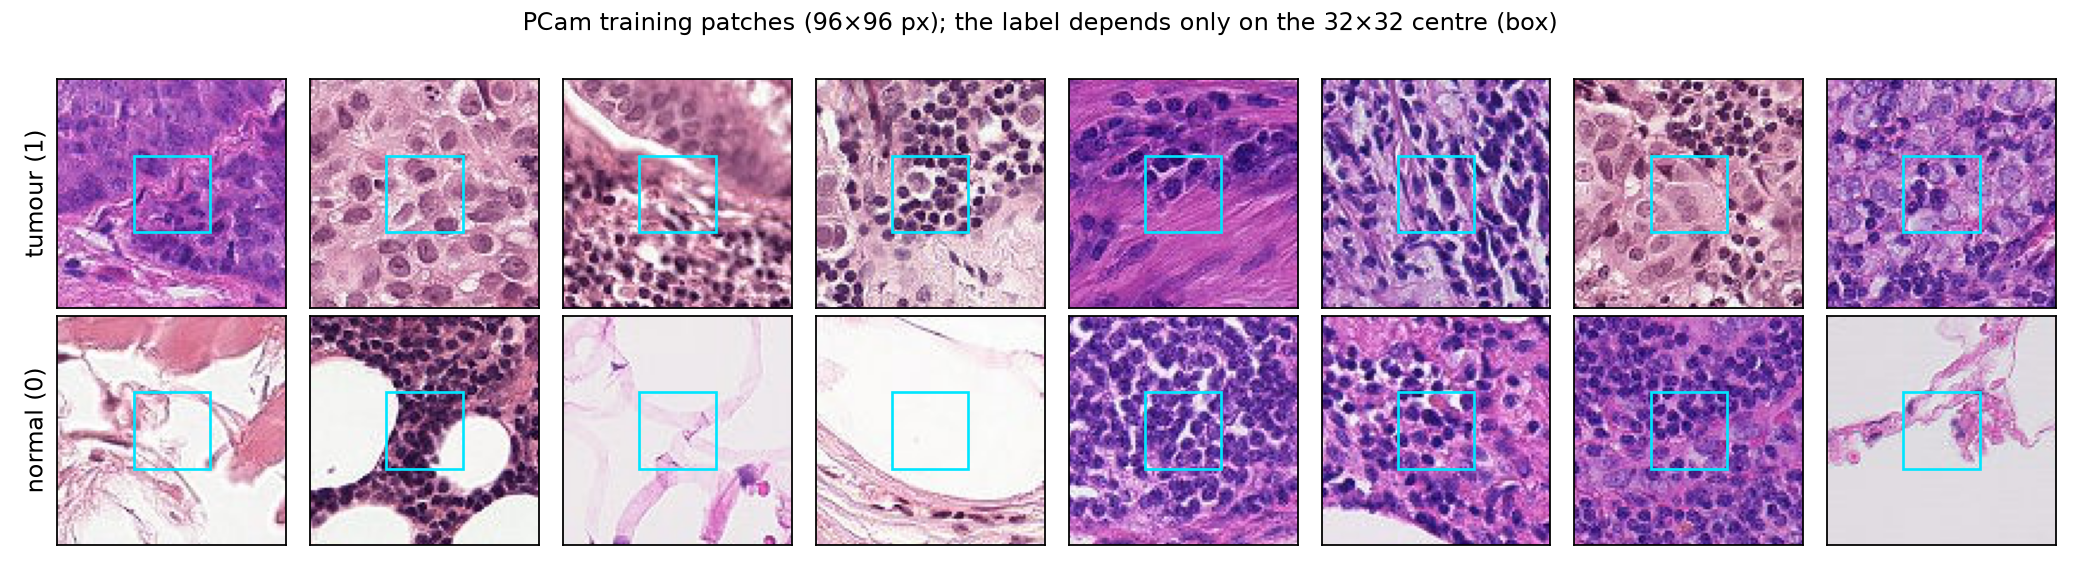
\includegraphics[width=\columnwidth]{fig_examples.png}
\caption{Random training patches. Top: tumour; bottom: normal. The label depends only on the boxed $32\times32$ centre.}
\label{fig:examples}
\end{figure}

\subsection{Data quality}
We audited all 327,680 records. \textit{Completeness:} no label or metadata field is missing, every image has the expected shape, and every label matches the metadata centre flag. \textit{Balance:} each split is 50/50, far above clinical prevalence, so accuracy and precision are optimistic. \textit{Duplicates:} hashing the pixels shows that 16.1\% of training patches are exact copies of another training patch (only 220,025 are unique), and 14.2\% and 10.3\% for validation and test; duplicates never disagree on the label. \textit{Leakage:} the splits are slide-disjoint by name, but test slide \texttt{test\_049} is the same physical slide as training slide \texttt{tumor\_036}: 36 patches share coordinates and pixels, and 285 of its 443 test patches overlap a training patch. We therefore also report test results without this slide. \textit{Label noise:} 673 training negatives (0.26\%) contain tumour outside the centre by design, and 173 positives are more than 90\% white background. \textit{Stain variation:} UMCU patches are darker than RUMC patches (mean haematoxylin optical density 0.044 vs.\ 0.031 after colour deconvolution~\cite{ruifrok2001}) and are more often positive (53\% vs.\ 48\%), so colour carries hospital information that is correlated with the label (Fig.~\ref{fig:stain}).

\begin{figure}[t]
\centering
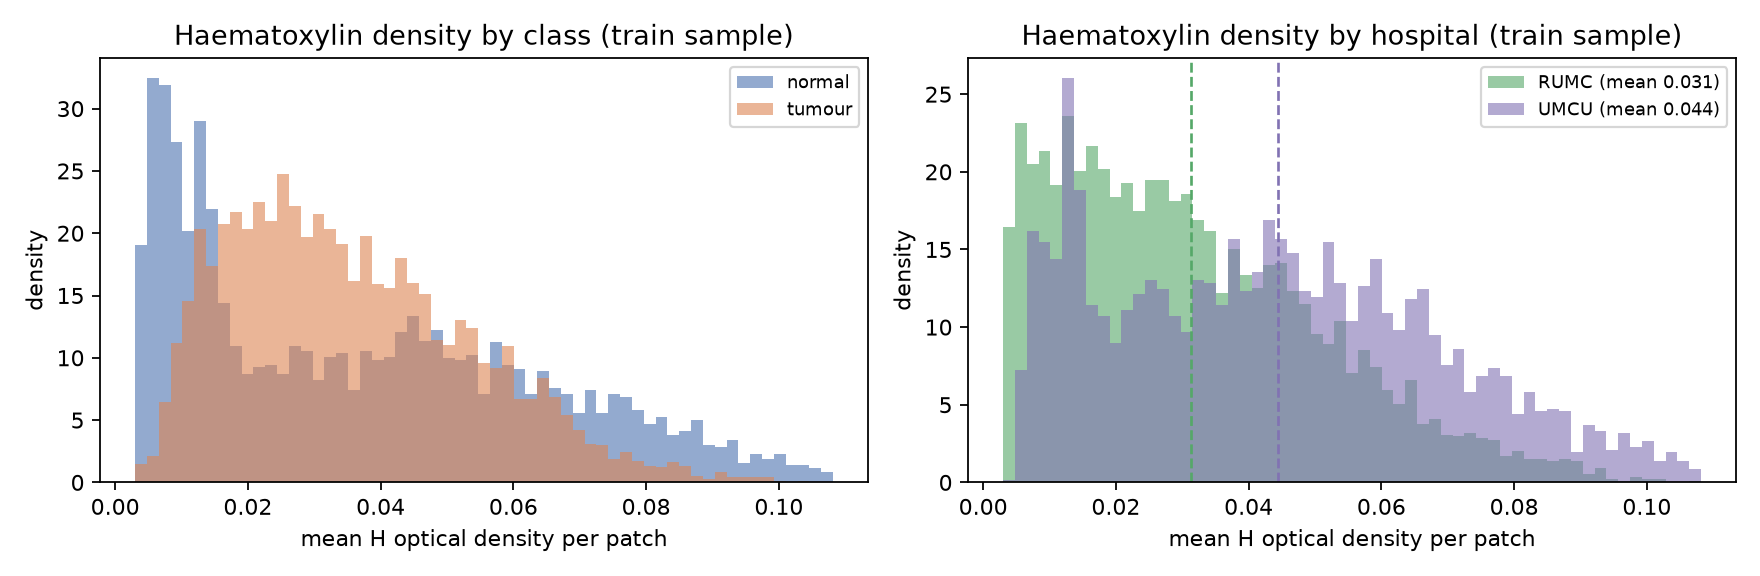
\includegraphics[width=\columnwidth]{fig_stain.png}
\caption{Haematoxylin optical density per patch (8,192 random training patches) by class (left) and by hospital (right).}
\label{fig:stain}
\end{figure}

\subsection{Preprocessing}
No imputation or cleaning was needed. We keep the duplicates in training so our numbers stay comparable with published PCam results, and we flag the leaked slide at evaluation. Pixels are scaled to $[0,1]$ and normalised with the ImageNet channel mean and standard deviation that the pretrained weights expect. Patches stay at their native $96\times96$ size. During training each patch gets a random element of the dihedral group (90° rotations and a horizontal flip); these 8 transforms are exact symmetries of tissue, keep the label centre in place and need no interpolation. We do not normalise stain, because RQ1 studies colour. The uint8 arrays are streamed once from HDF5 into GPU memory (8.2\,GB for train and validation) and batches are gathered there, which was 10$\times$ faster than random reads from disk on Colab.

\section{Baselines and Metrics}
\textit{Colour-only logistic regression.} Each patch is described by 58 colour features: the mean and standard deviation of R, G and B, of the haematoxylin and eosin optical densities~\cite{ruifrok2001}, and 16-bin histograms of each RGB channel. A standardised, L2-regularised logistic regression ($C=1$) is fitted on 32,768 random training patches. It sees no morphology, so it measures how much of the task colour alone explains.

\textit{ResNet-18.} A torchvision ResNet-18~\cite{he2016} (11.2M parameters) pretrained on ImageNet~\cite{deng2009}, with the classifier replaced by a single logit and trained with binary cross-entropy. We use AdamW~\cite{loshchilov2019} (learning rate $3\cdot10^{-4}$, weight decay $10^{-4}$), batch size 256, 10 epochs, 3\% linear warm-up then cosine decay, and mixed precision, on a \pending{GPU} in Colab (\pending{N} min). The checkpoint with the best validation AUC is evaluated once on test.

\textit{Metrics.} The main metric is ROC AUC, which does not depend on a threshold or on prevalence; its 95\% confidence interval comes from 1,000 bootstrap resamples of the test set. At a 0.5 threshold we also report accuracy, precision, recall (sensitivity), specificity and F1. Recall matters most clinically, since a missed metastasis is the costly error.

\section{Results}
\pending{Table~II and Fig.~3 go here once the ResNet-18 run finishes.}

\section{Analysis}
\pending{Interpretation goes here once the ResNet-18 run finishes.}

\begin{thebibliography}{9}
\bibitem{veeling2018} B. S. Veeling, J. Linmans, J. Winkens, T. Cohen, and M. Welling, ``Rotation equivariant CNNs for digital pathology,'' in \textit{Proc. MICCAI}, LNCS vol. 11071, 2018, pp. 210--218.
\bibitem{bejnordi2017} B. E. Bejnordi \textit{et al.}, ``Diagnostic assessment of deep learning algorithms for detection of lymph node metastases in women with breast cancer,'' \textit{JAMA}, vol. 318, no. 22, pp. 2199--2210, 2017.
\bibitem{litjens2018} G. Litjens \textit{et al.}, ``1399 H\&E-stained sentinel lymph node sections of breast cancer patients: the CAMELYON dataset,'' \textit{GigaScience}, vol. 7, no. 6, giy065, 2018.
\bibitem{ruifrok2001} A. C. Ruifrok and D. A. Johnston, ``Quantification of histochemical staining by color deconvolution,'' \textit{Anal. Quant. Cytol. Histol.}, vol. 23, no. 4, pp. 291--299, 2001.
\bibitem{he2016} K. He, X. Zhang, S. Ren, and J. Sun, ``Deep residual learning for image recognition,'' in \textit{Proc. IEEE CVPR}, 2016, pp. 770--778.
\bibitem{deng2009} J. Deng, W. Dong, R. Socher, L.-J. Li, K. Li, and L. Fei-Fei, ``ImageNet: A large-scale hierarchical image database,'' in \textit{Proc. IEEE CVPR}, 2009, pp. 248--255.
\bibitem{loshchilov2019} I. Loshchilov and F. Hutter, ``Decoupled weight decay regularization,'' in \textit{Proc. ICLR}, 2019.
\bibitem{tellez2019} D. Tellez \textit{et al.}, ``Quantifying the effects of data augmentation and stain color normalization in convolutional neural networks for computational pathology,'' \textit{Med. Image Anal.}, vol. 58, 101544, 2019.
\bibitem{komen2026} J. K\"omen \textit{et al.}, ``Towards robust foundation models for digital pathology,'' \textit{Nat. Commun.}, vol. 17, 5218, 2026.
\end{thebibliography}

\end{document}
